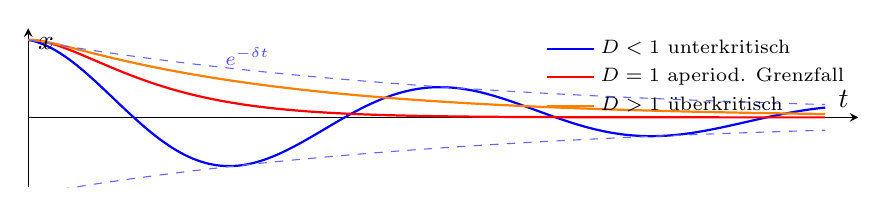
\begin{tikzpicture}
  \begin{axis}[
      width=\columnwidth, height=3.6cm,
      axis lines=middle, xmin=0, xmax=12.5, ymin=-0.9, ymax=1.15,
      xlabel={$t$}, ylabel={$x$}, ticks=none,
      samples=200, domain=0:12,
      legend style={font=\scriptsize, draw=none, fill=none, at={(1,1)}, anchor=north east},
      legend cell align=left,
    ]
    % omega_0 = 1, x(0) = 1, v(0) = 0
    \addplot[thick, blue]   {exp(-0.15*x)*cos(deg(0.989*x))};
    \addlegendentry{$D<1$ unterkritisch}
    \addplot[thick, red]    {(1+x)*exp(-x)};
    \addlegendentry{$D=1$ aperiod. Grenzfall}
    \addplot[thick, orange] {1.077*exp(-0.268*x) - 0.077*exp(-3.732*x)};
    \addlegendentry{$D>1$ überkritisch}
    \addplot[dashed, blue!60, forget plot] {exp(-0.15*x)};
    \addplot[dashed, blue!60, forget plot] {-exp(-0.15*x)};
    \node[blue!70, font=\scriptsize] at (axis cs:3.3,0.78) {$e^{-\delta t}$};
  \end{axis}
\end{tikzpicture}
